\documentclass[12pt]{article}

\usepackage{stoversymb,graphicx,soul}
\usepackage[letterpaper, margin=0.5in, top=0.75in, bottom=1in]{geometry}

\everymath{\displaystyle}

\usepackage{multicol}
\usepackage[many]{tcolorbox}
\usepackage{tikz}

\title{\vspace{-0.75in}\Huge{Areas of Various Regions Related to HW4~\#13(a)}\vspace{-0.5in}}
\date{}

\usepackage{array}
\newcolumntype{L}[1]{>{\raggedright\let\newline\\\arraybackslash\hspace{0pt}}m{#1}}
\newcolumntype{C}[1]{>{\centering\let\newline\\\arraybackslash\hspace{0pt}}m{#1}}
\newcolumntype{R}[1]{>{\raggedleft\let\newline\\\arraybackslash\hspace{0pt}}m{#1}}
\newcolumntype{N}{@{}m{0pt}@{}}

\usepackage[inline]{enumitem}
\setlist[enumerate,1]{leftmargin=0.5in, rightmargin=0.5in, label=(\roman*)}
\setlist[enumerate,2]{leftmargin=0.25in,label=(\alph*),itemsep=0.375in}

%\usepackage{caption,subcaption}
%	\captionsetup{subrefformat=parens}
%	\captionsetup{labelfont=bf,labelformat=simple,justification= centering,labelsep=newline,width=5.5in}
%	\captionsetup[figure]{belowskip=0px}
%	\captionsetup*[subfigure]{position=bottom}
	
\begin{document}
	\maketitle

	I wanted to give a complete answer to the problem(s) we discussed in class today (in particular, 13(a) and its hypothetical subparts). To do so, I'm going to work out full computations for the three possibilities.
	
	First, note that we had two curves: a circle $r=3$ and a cardioid $r=2(1+\cos{t})$. Those are shown in the below figure.
	
	\begin{tabular}{C{3.5in}C{3.5in}}
		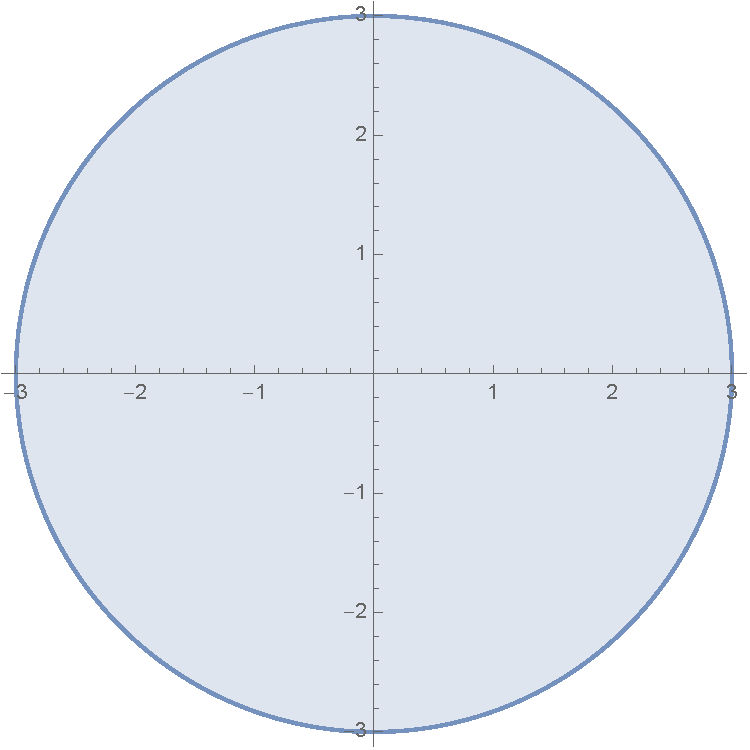
\includegraphics[height=2.75in]{circle} &
		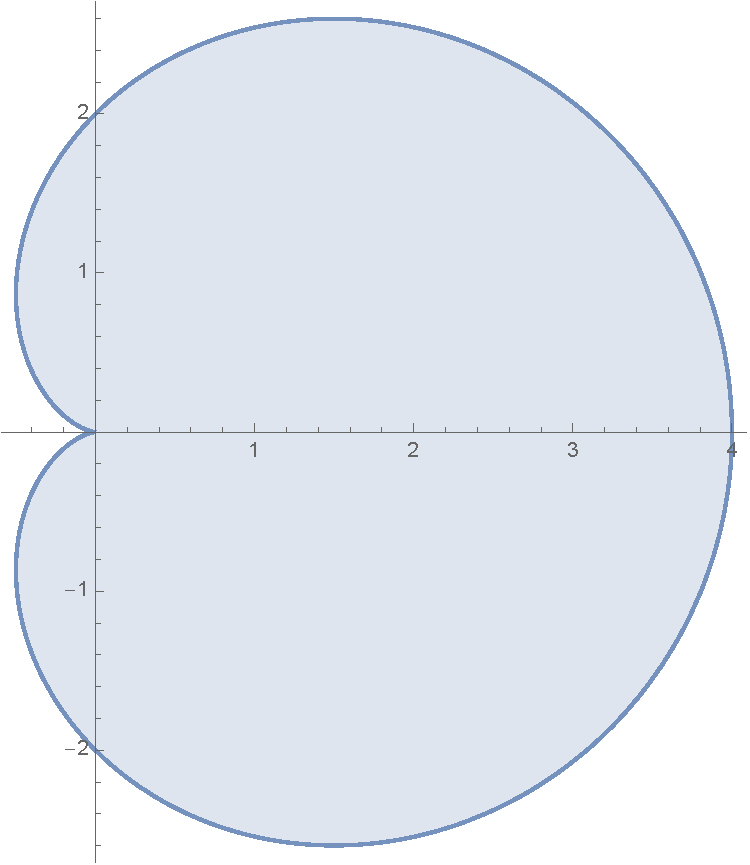
\includegraphics[height=2.75in]{cardioid}
	\end{tabular}

	\vspace{3mm}
	Before we start, let's find the area of the circle and the cardioid using the polar area formula:
	\vspace{-3mm}
	
	\begin{tabular}{C{2.75in}C{2.75in}}
	$$\begin{array}{rcl}
		A_{\text{circle}} & = &\frac{1}{2}\int_0^{2\pi}(3)^2\,d\theta\\[6mm]
			& = & \frac{1}{2}\int_0^{2\pi}9\,d\theta\\[6mm]
			& = & \frac{1}{2}\left(9\theta\,\Big|_0^{2\pi}\right)\\[6mm]
			& = & \frac{1}{2}\left(18\pi-0\right)\\[6mm]
			& = & 9\pi\\[1.75in]
		\end{array}$$
	&
	$$\begin{array}{rcl}
		A_{\text{cardioid}} & = & \frac{1}{2} \int_0^{2\pi}\left(2(1+\cos{\theta})\right)^2\,d\theta\\[6mm]
		& = & \frac{1}{2} \int_0^{2\pi}4(1+2\cos{\theta}+\cos^2{\theta})\,d\theta\\[6mm]
		& = & 2\int_0^{2\pi} 1 + 2\cos{\theta}+\cos^2{\theta}\,d\theta\\[6mm]
		& = &  2\int_0^{2\pi}1+2\cos\theta+\underbrace{\frac{1}{2}(1+\cos{2\theta})}_{\text{double angle formula}}d\theta\\[6mm]
		& = & 2\int_0^{2\pi} \frac{3}{2}+2\cos{\theta}+\frac{1}{2}\cos{2\theta}\,d\theta\\[6mm]
		& = & 2\left(\frac{3}{2}\theta + 2\sin\theta +\frac{1}{4}\sin{2\theta}\Bigg|_0^{2\pi}\right)\\[7.5mm]
		& = & 2\left(3\pi + 0 + 0 - 0 - 0 - 0\right)\\[6mm]
		& = & 6\pi
	\end{array}$$
	\end{tabular}

	\noindent Next, before we look at the regions specific to \#13(a), we should note/clarify a couple things:
	\begin{enumerate}
		\item You \textbf{always} want to choose your $\theta$ values in a \textbf{counterclockwise fashion}, increasing from \textbf{smaller} to \textbf{larger}.
		\item The choice of \textbf{outer curve} and \textbf{inner curve} will depend on the figures in question and on the regions you're shading in. 
	\end{enumerate}

	\begin{tcolorbox}[enhanced,colback=white,colframe=black,boxrule=0.5pt,arc=0pt,top=3mm,bottom=3mm]
		\noindent\red{\textbf{Note on (2):} The thing we discussed in class about ``reading from left-to-right and/or bottom-to-top'' was a \textit{heuristic} which \textit{fit the example we were doing} but which \textit{\textbf{isn't always true}}!} 
		
		\vspace{3mm}
		
		\textbf{In general:} Your outer curve will be the one which bounds your region and which has the \textbf{largest absolute value}!
	\end{tcolorbox}

	\vspace{3mm}
	
	As we saw in class, the curve $r=3$ intersects the curve $r=2(1+cos\theta)$ at the points $\theta=\pi/3$ and $\theta=5\pi/3$. Note here that the ray $\theta=5\pi/3$ is the same as the ray $\theta=-\pi/3$, and this is a fact we'll use a bit later.
	
	Now, let's look at the three possibilities stemming from \#13~(a).\\[1.5mm]
	
	\noindent\textbf{Possibility 1: The Leftmost Region}
	
	\begin{center}
		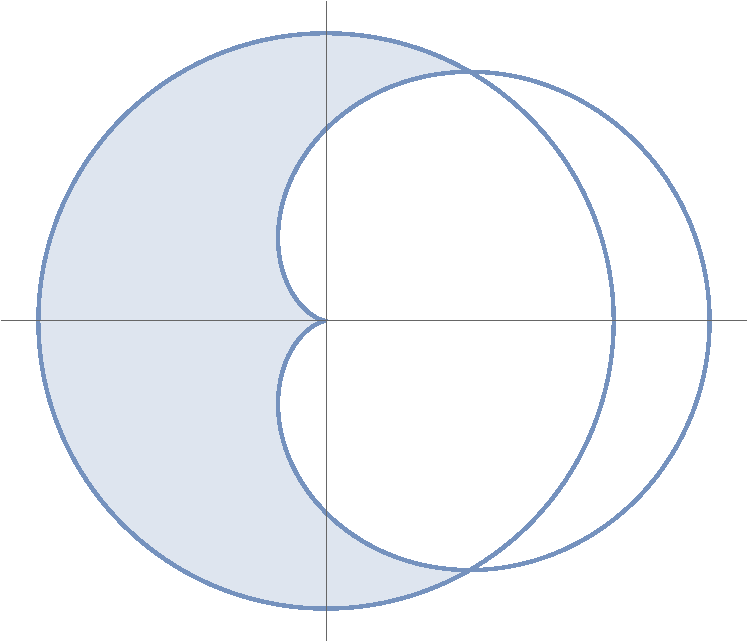
\includegraphics[scale=0.75]{region1}
	\end{center}

	This is the example we did in class (and which is on the homework).
	
	\begin{itemize}
		\item \ul{Finding $\theta$:}  Note that traversing either curve (the circle, say) in the standard counterclockwise fashion will trace the region as $\theta$ ranges from $\pi/3$ to $5\pi/3$. Because $\pi/3 < 5\pi/3$, this is the range we'll use.
		\item \ul{Finding outer/inner curves:} Note that the leftmost point on the portion of the circle bounding the region is $(-3,0)$, while the leftmost point on the portion of the cardioid bounding the shaded region is between that and the ``$y$-axis''. 
		
		In particular, the absolute value of the circle point is larger than the absolute value of the cardioid point, and so: \textbf{Outer curve = circle} and \textbf{inner curve = cardioid}.
	\end{itemize} 

	Now, to find the area:
	$$\begin{array}{rcl}
		A_{\text{leftmost}} & = & \frac{1}{2}\int_{\pi/3}^{5\pi/3}(r_{\text{outer}})^2-(r_{\text{inner}})^2\,d\theta\\[6mm]
		 & = & \frac{1}{2} \int_{\pi/3}^{5\pi/3}\left(3^2 - (2(1+\cos{\theta}))^2\right)\,d\theta\\[6mm]
		 & = & \frac{1}{2} \int_{\pi/3}^{5\pi^3}9-4(1+2\cos{\theta}+\cos^2\theta)\,d\theta\text{\quad\,\, (by squaring each expression)}\\[6mm]
		 & = & \frac{1}{2} \int_{\pi/3}^{5\pi/3}5-8\cos\theta-2\left(1+\cos{2\theta}\right)\,d\theta\text{\quad (using double-angle)}\\[6mm]
		 & = & \frac{1}{2} \int_{\pi/3}^{5\pi/3}3-8\cos\theta-2\cos{2\theta}\,d\theta\\[6mm]
		 & = & \frac{1}{2} \left(3\theta -8\sin{\theta}-\sin{2\theta}\,\Bigg|_{\pi/3}^{5\pi/3}\right)\\[6mm]
		 & = & \frac{1}{2} \left(5\pi+4\sqrt{3}+\frac{\sqrt{3}}{2}-\pi+4\sqrt{3}+\frac{\sqrt{3}}{2}\right)\\[6mm]
		 & = & \frac{9\sqrt{3}}{2}+2\pi.
	\end{array}$$
	
	\vspace{3mm}
	
	\noindent\textbf{Possibility 2: The Rightmost Region (``The Sliver'')}
	
	We talked about this one briefly, but it wasn't very precise.
		
	\begin{center}
		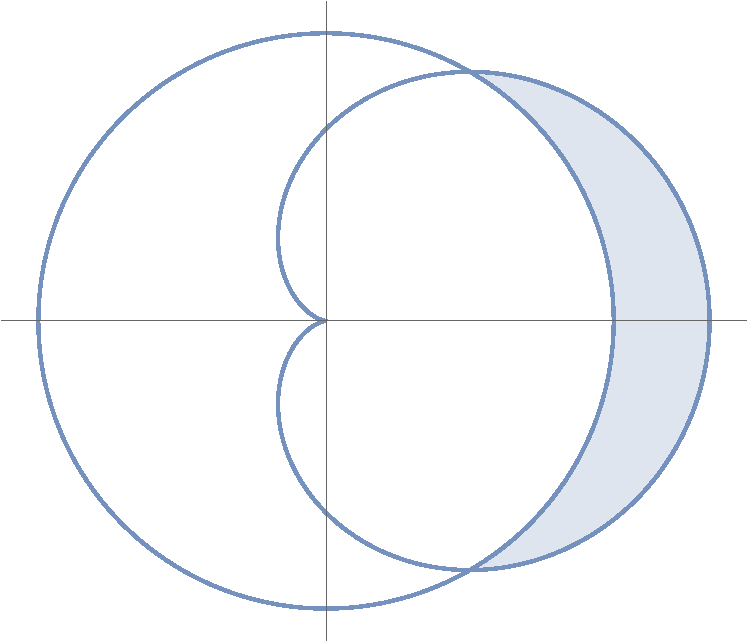
\includegraphics[scale=0.75]{region3}
	\end{center}
	
	\begin{itemize}
		\item \ul{Finding $\theta$:} Because the region in Possibility 1 is traced from $\theta=\pi/3$ to $\theta=5\pi/3$, the obvious deduction for this region is that $\theta$ goes from $5\pi/3$ to $\pi/3$. This is right \textbf{in principle}, but remember: You want $\theta$ to be \textbf{increasing}. 
		
		Therefore, since $5\pi/3 > \pi/3$, we swap $5\pi/3$ for $-\pi/3$  and let $\theta$ range from $-\pi/3$ to $\pi/3$ to get increasing values of $\theta$.
		
		\item \ul{Finding outer/inner curves:} Here, note that the rightmost point on the portion of the cardioid bounding the region is $(4,0)$, while the rightmost point on the portion of the circle bounding the region is $(3,0)$.
		
		Thus, the rightmost circle point is between the rightmost cardioid point and the ``$y$-axis,'' thus making the absolute value of the cardioid point larger and implying: \textbf{Outer curve = cardioid} and \textbf{inner curve = circle}.
	\end{itemize} 

	As for the area
	$$\begin{array}{rcl}
	A_{\text{sliver}} & = & \frac{1}{2}\int_{-\pi/3}^{\pi/3}(r_{\text{outer}})^2-(r_{\text{inner}})^2\,d\theta\\[6mm]
	& = & \frac{1}{2} \int_{-\pi/3}^{\pi/3}\left( (2(1+\cos{\theta}))^2-3^2 \right)\,d\theta\\[6mm]
	& = & \frac{1}{2} \int_{-\pi/3}^{\pi/3}4(1+2\cos{\theta}+\cos^2\theta)-9\,d\theta\text{\quad\,\, (by squaring each expression)}\\[6mm]
	& = & \frac{1}{2} \int_{-\pi/3}^{\pi/3}-5+8\cos\theta+2\left(1+\cos{2\theta}\right)\,d\theta\text{\quad (using double-angle)}\\[6mm]
	& = & \frac{1}{2} \int_{-\pi/3}^{\pi/3}-3+8\cos\theta+2\cos{2\theta}\,d\theta\\[6mm]
	& = & \frac{1}{2} \left(-3\theta +8\sin{\theta}+\sin{2\theta}\,\Bigg|_{-\pi/3}^{\pi/3}\right)\\[6mm]
	& = & \frac{1}{2} \left(-\pi+4\sqrt{3}+\frac{\sqrt{3}}{2}-\pi+4\sqrt{3}+\frac{\sqrt{3}}{2}\right)\\[6mm]
	& = & \frac{9\sqrt{3}}{2}-\pi.
	\end{array}$$
	
	\vspace{3mm}
	
	\noindent\textbf{Possibility 3: The Middle Region (``The Inside'')}
	This one is saved for the end because it's different than the others.
	
	In particular, note that because $\pi/3\rightarrow5\pi/3$ bounds the first region and $5\pi/3(=-\pi/3)\rightarrow\pi/3$ bounds the second, there are no values of $\theta$ which we can use to bound the region in the middle. Thus, we have to get a bit clever to find the area $A_{\text{inside}}$.
	
	``Clever'' can take one of two forms depending on which of the following facts you observe first:

	\begin{enumerate}
		\item $A_{\text{circle}}=A_{\text{leftmost}}+A_{\text{inside}}\implies A_{\text{inside}}=A_{\text{circle}}-A_{\text{leftmost}}.$
		\item $A_{\text{inside}}+A_{\text{sliver}}=A_{\text{cardioid}}\implies A_{\text{inside}}=A_{\text{cardioid}}-A_{\text{sliver}}.$
	\end{enumerate}

	\begin{center}
		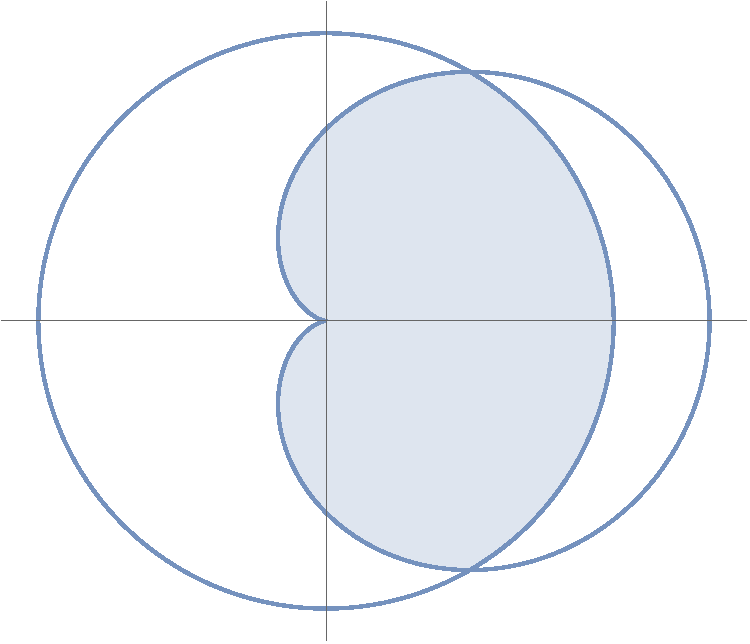
\includegraphics[scale=0.75]{region2}
	\end{center}

	\noindent Now, because we know $A_{\text{circle}}=9\pi$, $A_{\text{cardioid}}=6\pi$, 
	$$A_{\text{leftmost}}=\frac{9\sqrt{3}}{2}+2\pi\quad\text{ and }\quad A_{\text{sliver}}=\frac{9\sqrt{3}}{2}-\pi,$$ we have two different formulas for finding $A_{\text{inside}}$:
	$$A_{\text{inside}}=A_{\text{circle}}-A_{\text{leftmost}}\implies A_{\text{inside}}=9\pi-\left(\frac{9\sqrt{3}}{2}+2\pi\right)=7\pi-\frac{9\sqrt{3}}{2},$$
	and
	$$A_{\text{inside}}=A_{\text{cardioid}}-A_{\text{sliver}}\implies A_{\text{inside}}=6\pi-\left(\frac{9\sqrt{3}}{2}-\pi\right)=7\pi-\frac{9\sqrt{3}}{2}.$$
	
	From this, we can also find the total area bounded by all the regions:
	$$\begin{array}{rcl}
		A_{\text{total}} 
			& = & A_{\text{leftmost}} + A_{\text{inside}} + A_{\text{sliver}} \\[6mm]
			& = & \frac{9\sqrt{3}}{2}+2\pi + 7\pi-\frac{9\sqrt{3}}{2} + \frac{9\sqrt{3}}{2}-\pi \\[6mm]
			& = & \frac{9\sqrt{3}}{2}+8\pi.
	\end{array}$$
		
\end{document}